\chapter*{Conclusion: Part~\ref{part:cosmology}}
\addcontentsline{toc}{chapter}{Conclusion: Part~\ref{part:cosmology}}
\markboth{Conclusion: Part~\ref{part:cosmology}}{Conclusion: Part~\ref{part:cosmology}}

This part began by showing in Chapter~\ref{chap:kd} that almost all classical inflationary solutions begin in a generic kinetically dominated phase. The generality of this statement was discussed in Chapter~\ref{chap:kt}. 
Whether or not this phase occurs in reality can only be established by observation. If inflation was sufficiently short, then this pre-inflationary epoch may be observable as a suppression in power at low-$\ell$ in the $C_\ell$ spectrum, or in low-$k$ in the $\mathcal{P}_\mathcal{R}(k)$ spectrum. 

In Chapter~\ref{chap:rec}, I showed that if one reconstructs the primordial power spectrum $\mathcal{P}_\mathcal{R}(k)$ from a Bayesian perspective there is some weak evidence for a suppression of power at low-$k$, as well as an anomaly at $\ell\sim30$. Whilst this by no means provides evidence for an observable kinetically dominated epoch, it does suggest the possibility that with better data there could be.

In order to gain more theoretical guidance on the precise predictions which the kinetically dominated universe makes about the primordial power spectrum, we have to gain a greater understanding of the quantum mechanics of this phase. The details of this are non-trivial, since as soon as one migrates away from a de-Sitter limit, the theory as to how to set initial conditions becomes far more murky. Chapter~\ref{chap:qv} has enumerated some of these issues, and provided an alternative possibility for quantising a kinetically dominated universe.

\section*{Future work}
\subsection*{Theoretically investigating kinetically dominance}
The results of Chapter~\ref{chap:kt} require further investigation. In particular, since linear spatial perturbations grow backwards in time, the universe is more inhomogeneous closer to $t=0$. This will lead to a breakdown in the assumptions at some point, and it would be helpful to quantify this fully. In particular, it would useful to know if the breakdown is earlier than the Planck scale for $k$-scales of observational interest.

Further, since the kinetically dominated universe stabilises forwards in time, it would be interesting to quantify how generic our initial conditions are, and whether a homogeneous kinetically dominated phase naturally arises for any universe beginning with $\dot{\phi}^2\gg V(\phi)$. This would involve similar machinery to that used in ``eternal inflation'' scenarios.


\subsection*{Constraining the kinetically dominated universe}

The next task would be to ask if the data can provide any further insight into the quantum vacuum of the kinetically dominated universe. It would be particularly interesting to find out if the data themselves were capable of distinguishing between vacua. This could be done for the current set of cosmological data, or one could ask about the feasibility of future data sets in providing constraints on this portion of the unierse.

A full analysis would involve numerically integrating the quantum mechanical equations through the pre-inflationary phase all the way to horizon exit. Since these equations are highly oscillatory with time-varying coefficients, this would require a numerical method capable of tackling these. In fact, I have begun work on such a technique, which is detailed in Chapter~\ref{chap:RK}.

If one of these vacua is the ``correct'' one, it still remains to be determined when, if at all, it was in its vacuum state. It may be that we can provide observational constraints on the precise value of this moment.

\subsection*{Further constraints on inflation}
In addition, as a member of Planck core team II, I intend to continue more traditional observational reconstructions of inflationary and cosmological functions.

In general, inflationary analysis begins with the definition of the potential $V(\phi)$. This then predicts a primordial power spectrum $\mathcal{P}_\mathcal{R}(k)$ via a numerical integration of the Mukhanov-Sazaki (MS) equations. The primordial power spectrum is then converted via cosmological transfer functions ($\Delta$) into a set of multipole moments:

\tikzsetnextfilename{inflation_procedure}
\begin{center}
  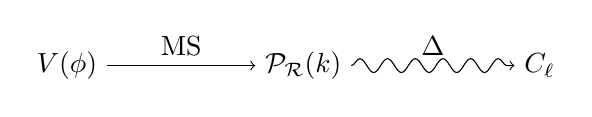
\begin{tikzpicture}[decoration=snake]
    \draw[] (3,0) node (Cl) {$C_\ell$};
    \draw[] (0,0) node (Pr) {$\mathcal{P}_\mathcal{R}(k)$};
    \draw[] (-3,0) node (Vphi) {$V(\phi)$};
    \draw[->,decorate] (Pr) -- (Cl) node[midway,above]{$\Delta$};
    \draw[->] (Vphi) -- (Pr) node[midway,above]{MS};
  \end{tikzpicture}
\end{center}

In Chapter~\ref{chap:rec} we applied a Bayesian reconstruction procedure to the middle stage, and reconstructed the primordial power spectrum in a model independent manner.  
We intend to apply our Bayesian reconstruction procedure separately to all three of these stages of the analysis, with the new updated polarisation data.

%\subsubsection{Primordial power spectrum $\mathcal{P}_\mathcal{R}(k)$ reconstruction}
%This would be much the same as in the 2015 paper, with possibly a little more investigation into prior sensitivities, and obviously updated to use the new polarisation data.
%
%\subsubsection{Inflationary potential $V(\phi)$ reconstruction}
%Here we would parameterise the inflationary potential $V(\phi)$ with movable knots. In addition, we will require the e-folding of the pivot scale $50<N_*<60$ to be a free parameter to be fitted. This avoids any difficulties with re-heating parameterisations.
%To avoid ``ringing'' effects in the subsequent primordial power spectrum, we will probably use a cubic rather than linear spline. We will also put a fairly strong prior on the potential; 
%\begin{itemize}
%  \item Inflation must finish at $\phi=0$. This can be achieved by setting $V=\frac{d}{d\phi}V = 0$ at $\phi=0$.
%  \item The potential must support at least $50-60$ e-folds of inflation, with a continuous inflationary phase in between $\phi=\phi_*$ and $\phi=0$.
%\end{itemize}
%For this reason, it is essential that we provide plots of the prior $V(\phi)$ as well as the posterior.
%
%The horizontal prior on the $\phi$-co\"{o}rdinates of the knots will be linear, whilst the prior on the vertical position will be either logarithmic or linear (we will attempt both).
%
%\subsubsection{Multipole moment $C_\ell$ reconstruction}
%Here, the aim is to move the reconstruction to the other end of the analysis, and probe the significance of the anomalies (if any) that have been appearing in the $C_\ell$ spectrum. 
%
%The Planck likelihoods may be thought of as functions of the theoretical multipole moments $C_\ell^\mathrm{\Lambda CDM}$, which are in turn functions of the $\Lambda$CDM cosmological parameters $\Theta$:
%\begin{equation}
%  \mathcal{L} = \mathcal{L}(C_\ell), \qquad C_\ell = C_\ell^{\mathrm{\Lambda CDM}}(\Theta)
%\end{equation}
%  
%  Our plan is to parameterise the theoretical $C_\ell$'s with an additional reconstructed alteration:
%\begin{equation}
%  C_\ell = C_\ell^\mathrm{\Lambda CDM}(\Theta) + \delta C_\ell(\Psi),
%\end{equation}
%where $\Psi$ are a set of reconstruction parameters for the unknown function.
%
%Priors on the $\delta C_\ell$ and $\ell$ components of the knots will have to be considered carefully, but a parameterisation that is linear in $\ell(\ell+1)\delta C_\ell$ and $\ell$ seems a reasonable start. We may also need to discretise the $\ell$-positions of the knots. There is nothing about our analysis (or \PolyChord{}) that precludes this option. 
%
%It would also be useful to see the equivalent plots of Figure~\ref{fig:full_bayes_knots} for the $C_\ell$'s in comparison to their observed values and errors.
%
%One particularly powerful aspect of this parameterisation, is that the $\delta C_\ell$ adjustment occurs post-transfer function calculation. This means that $\Psi$ are effectively ``fast parameters'', and we can therefore potentially add a great many of these before incurring a computational cost.
%
%
%
\cleardoublepage{}
